\section{Experimental Results}

\subsection{Grammar and Model Generation}
\label{section-grammar-model-timing}

%         NB class GrammarModelTiming

The first experiment set will try to establish how long it takes to extract the IG % TODO IG -> nomenclature
from the input XML file and how long does it take to create the AM model from this IG. For now, we will not be running or measuring any heuristics.

\begin{center}
\bigskip
\begin{tabular}{| l | l |}
  \hline
  \hline
  Input data        & all official and sized test data sets \\
  Iterations        & 50 \\
  Pool size         & not applicable \\
  $\alpha$, $\beta$ & not applicable \\
  CH                & not applicable \\
  IHs               & not applicable \\
  \hline
\end{tabular}
\bigskip
\end{center}

The experimental set will contain $50 * (11 + 11) = 1100$ configurations: 50 iterations for 11 test data sets plus 11 sized test data sets. There will be no CHs or IHs. We will be gathering the timing data for IG extraction and model generation in GnuPlot format.\\

\begin{table}
  \caption{Grammar Extraction and Model Creation Times}
  \bigskip
  \label{table-experiments-grammar-model-timing}
  \centering
  \begin{tabular}{l || l | l || l | l || l | l}
    Data set & GE & GE & MC & MC & Tot & Tot \\
     & avg [ms] & stdev & avg [ms] & stdev & avg [ms] & stdev \\
    \hline
    \dataset{OVA1}     & < 10 & - & < 10 & - & < 10 & - \\
    \dataset{OVA2}     & < 10 & - & < 10 & - & < 10 & - \\
    \dataset{OVA3}     & 42.94 & 19.8509 & 60.92 & 27.0848 & 103.86	& 31.6911 \\
    \dataset{XMA-c}    & 140.32 &	33.2618 &	90.24 &	45.8803 & 230.56 & 56.2633 \\
	\dataset{XMA-p}    & 7518.82 &	922.8882 &	10135.46 &	502.8997 & 17654.28	& 1353.8794 \\
	\dataset{XMD}      & 979.18 &	307.1760 &	563.04 & 341.4697 & 1542.22	& 134.6883 \\
	\dataset{MSH}      & 570.24 &	167.1119 &	225.48 &	90.6775 & 795.72 & 161.8340 \\ 
	\dataset{NTH}      & 328.36 & 118.3766 &	1074.9 &	155.5604 & 1403.26 & 137.8695 \\
	\dataset{100-100}  & < 10 & - & < 10 & - & < 10 & - \\
	\dataset{100-200}  & < 10 & - & < 10 & - & < 10 & - \\
	\dataset{100-1000} & 18.34 & 10.2372 & 18.84 & 1.0373 & 37.18 & 9.9338 \\
	\dataset{0-0}      & < 10 & - & < 10 & - & < 10 & - \\
	\dataset{10-5}     & < 10 & - & < 10 & - & < 10 & - \\
	\dataset{20-20}    & < 10 & - & < 10 & - & < 10 & - \\
	\dataset{30-45}    & < 10 & - & < 10 & - & < 10 & - \\
	\dataset{40-80}    & < 10 & - & < 10 & - & < 10 & - \\
	\dataset{50-125}   & < 10 & - & < 10 & - & < 10 & - \\
	\dataset{60-180}   & < 10 & - & < 10 & - & < 10 & - \\
	\dataset{70-245}   & < 10 & - & < 10 & - & < 10 & - \\
	\dataset{80-320}   & < 10 & - & < 10 & - & 12.48 & 8.3574 \\
	\dataset{90-405}   & < 10 & - & < 10 & - & 15.88 & 10.3778 \\
	\dataset{100-500}  & < 10 & - & < 10 & - & 18.74 &	8.8889 \\
  \end{tabular}
\end{table}

Results are in Table \ref{table-experiments-grammar-model-timing}. We are presenting the average grammar extraction (GE) times and their standard deviation, the same for model creation (MC) and total (sum of these two, Tot) times. For many data sets the average time is less than 10 ms: this is not enough to be precise and we don't calculate the standard deviation in these cases.

We can see from the results that for most data sets their model can easily be created under around one second, only in case of the biggest set \dataset{XMA-p} (13 MB) this takes some 17 seconds. We can conclude that grammar and model creation times are not a bottleneck for now. Heuristics run times will be order of magnitude higher.

\subsubsection{GLPK Interface Timing}

%         NB class GlpkInterfaceTiming

A related problem is how long it takes to create input for GLPK and then parse its results. We will use the same test data sets as in the previous case, but now we will gather times needed to communicate with GLPK.\\

\begin{table}
  \caption{GLPK Interface Times}
  \bigskip
  \label{table-experiments-glpk-timing}
  \centering
  \begin{tabular}{l || l | l || l | l || l | l}
	Data set & IC & IC & OP & OP & Tot & Tot \\
     & avg [ms] & stdev & avg [ms] & stdev & avg [ms] & stdev \\
	\hline
	\dataset{OVA1} & 36.46 & 66.8517 & 49.8 & 114.0687 & 86.26 & 150.1044 \\
	\dataset{OVA2} & 39.52 & 75.8210 & 48.8 & 102.4484 & 88.32 & 154.9596 \\
	\dataset{OVA3} & 34.1 & 74.1838 & 38.62 & 89.3772 & 72.72 & 134.7295 \\
	\dataset{XMA-c} & 40.88 & 88.6632 & 33.84 & 65.8636 & 74.72 & 127.7338 \\
	\dataset{XMA-p} & 36.54 & 70.7436 & 49.24 & 101.2412 & 85.78 & 145.2092 \\
	\dataset{XMD} & 37.98 & 69.2719 & 32.88 & 70.2173 & 70.86 & 114.6692 \\
	\dataset{MSH} & 40.42 & 91.9885 & 36.52 & 72.1018 & 76.94 & 138.6198 \\
	\dataset{NTH} & 36.02 & 66.3403 & 38.06 & 88.8244 & 74.08 & 128.9974 \\
	\dataset{100-100} & 46.5 & 103.3929 & 46.92 & 89.7049 & 93.42 & 158.7267 \\
	\dataset{100-200} & 42.34 & 96.1204 & 38.22 & 90.0284 & 80.56 & 152.6534 \\
	\dataset{100-1000} & 32.92 & 64.4534 & 42.1 & 89.4546 & 75.02 & 127.8541 \\
	\dataset{0-0} & 46.8 & 123.5183 & 46.92 & 102.2601 & 93.72 & 181.5228 \\
	\dataset{10-5} & 40.06 & 75.7370 & 40.1 & 72.4851 & 80.16 & 126.7135 \\
	\dataset{20-20} & 33.72 & 70.7263 & 34.1 & 66.2781 & 67.82 & 116.3783 \\
	\dataset{30-45} & 38.26 & 71.7549 & 45.94 & 110.1284 & 84.2 & 155.7594 \\
	\dataset{40-80} & 37.06 & 67.0024 & 49.26 & 106.3185 & 86.32 & 144.9918 \\
	\dataset{50-125} & 50.44 & 101.9162 & 84.76 & 364.7350 & 135.2 & 378.7835 \\
	\dataset{60-180} & 38.38 & 89.3379 & 42.54 & 94.3742 & 80.92 & 149.6049 \\
	\dataset{70-245} & 41.5 & 93.2951 & 40.3 & 93.4858 & 81.8 & 149.6797 \\
	\dataset{80-320} & 51.92 & 121.9812 & 47.98 & 96.0904 & 99.9 & 171.4617 \\
	\dataset{90-405} & 40.5 & 91.5373 & 36.46 & 88.5099 & 76.96 & 144.2890 \\
	\dataset{100-500} & 37.82 & 85.7571 & 43.4 & 90.3257 & 81.22 & 141.9103 \\
  \end{tabular}
\end{table}

Results are in table \ref{table-experiments-glpk-timing}. For each data set there are the times of (GLPK) input creation (IC) - average and standard deviation, then the same for output parsing (OP) and total (Tot).

Interestingly enough, in most cases the times to create an input for GLPK and then to parse its output are very similar. Also, for sized test data sets it is interesting to note that even though the $|V|$ and $|E|$ counts are increasing, the times remain almost the same. This probably due to the fact that IC and OP times include the I/O when writing to a file for GLPK or reading the file it produced, and these times are probably the most relevant.

\subsection{GLPK: Native vs. Cygwin}

%         NB class TimeQuality
%         NB class TimeTillOptimum

In this experiment we will try to remove one of the variables out of the equation: that is the effect of different versions of GLPK on the overall results. The rationale is this: on Windows systems, the two most accessible ways to install GLPK are via a binary distribution, % TODO link
or via Cygwin as one of its packages.

If we find out which of these Cygwin version is better, we will be using it exclusively knowing this should not affect any other aspect of our experiments. We might also find that there is no relevant difference, which would be and interesting finding, too.

Apart from comparing different versions, we shall see how the pure GLPK approach behaves. The first part of this experiment will be limiting the run time, thus making it an instance of \heu{Truncated branch \& bound}. In this case we will see the dependency between the run time and the quality achieved in it. In the second time we will let GLPK run until optimum is found. We shall see the dependency between input size and run time needed to achieve the optimum.

\begin{center}
\bigskip
\begin{tabular}{| l | l |}
  \hline
  \hline
  Input data        & \dataset{100-500} \\
  Iterations        & 50 \\
  Pool size         & 1 \\
  $\alpha$, $\beta$ & $1$, $1$ \\
  CH                & \heu{Glpk} \\
  IHs               & $\emptyset$ \\
  \hline
\end{tabular}
\bigskip
\end{center}

Our experimental set will contain 500 experimental configurations for each of these two GLPK version. Every configuration will use \heu{Glpk} CH set to a time limit from 1 to 46 seconds with increments of 5, meaning 10 settings * 50 iterations = 500 configurations in total (see Listing \ref{listing-experiment-glpk-native-vs-cygwin-1}). There will be no improvement heuristic. The only data we gather in the GnuPlot file are the final qualities (weights). The data set used is \dataset{100-500} as the biggest one in sized test data.\\

\begin{algorithm}
\caption{GLPK: Native vs. Cygwin Set Generation 1}
\label{listing-experiment-glpk-native-vs-cygwin-1}
\begin{algorithmic}
\ENSURE experimental set $ES$
\STATE $ES \gets \emptyset$
\FOR{$i = 1 \to 50$}
	\FOR{$time = 1 \to 46$ step $5$}
    \STATE $ES \gets ES \cup {CH = \heu{Glpk}(limit = time), IH = \emptyset}$
  \ENDFOR
\ENDFOR
\RETURN $ES$
\end{algorithmic}
\end{algorithm}

\begin{figure}
  \caption{Time vs. Quality}
  \label{image-experiment-time-vs-quality}
  \centering
    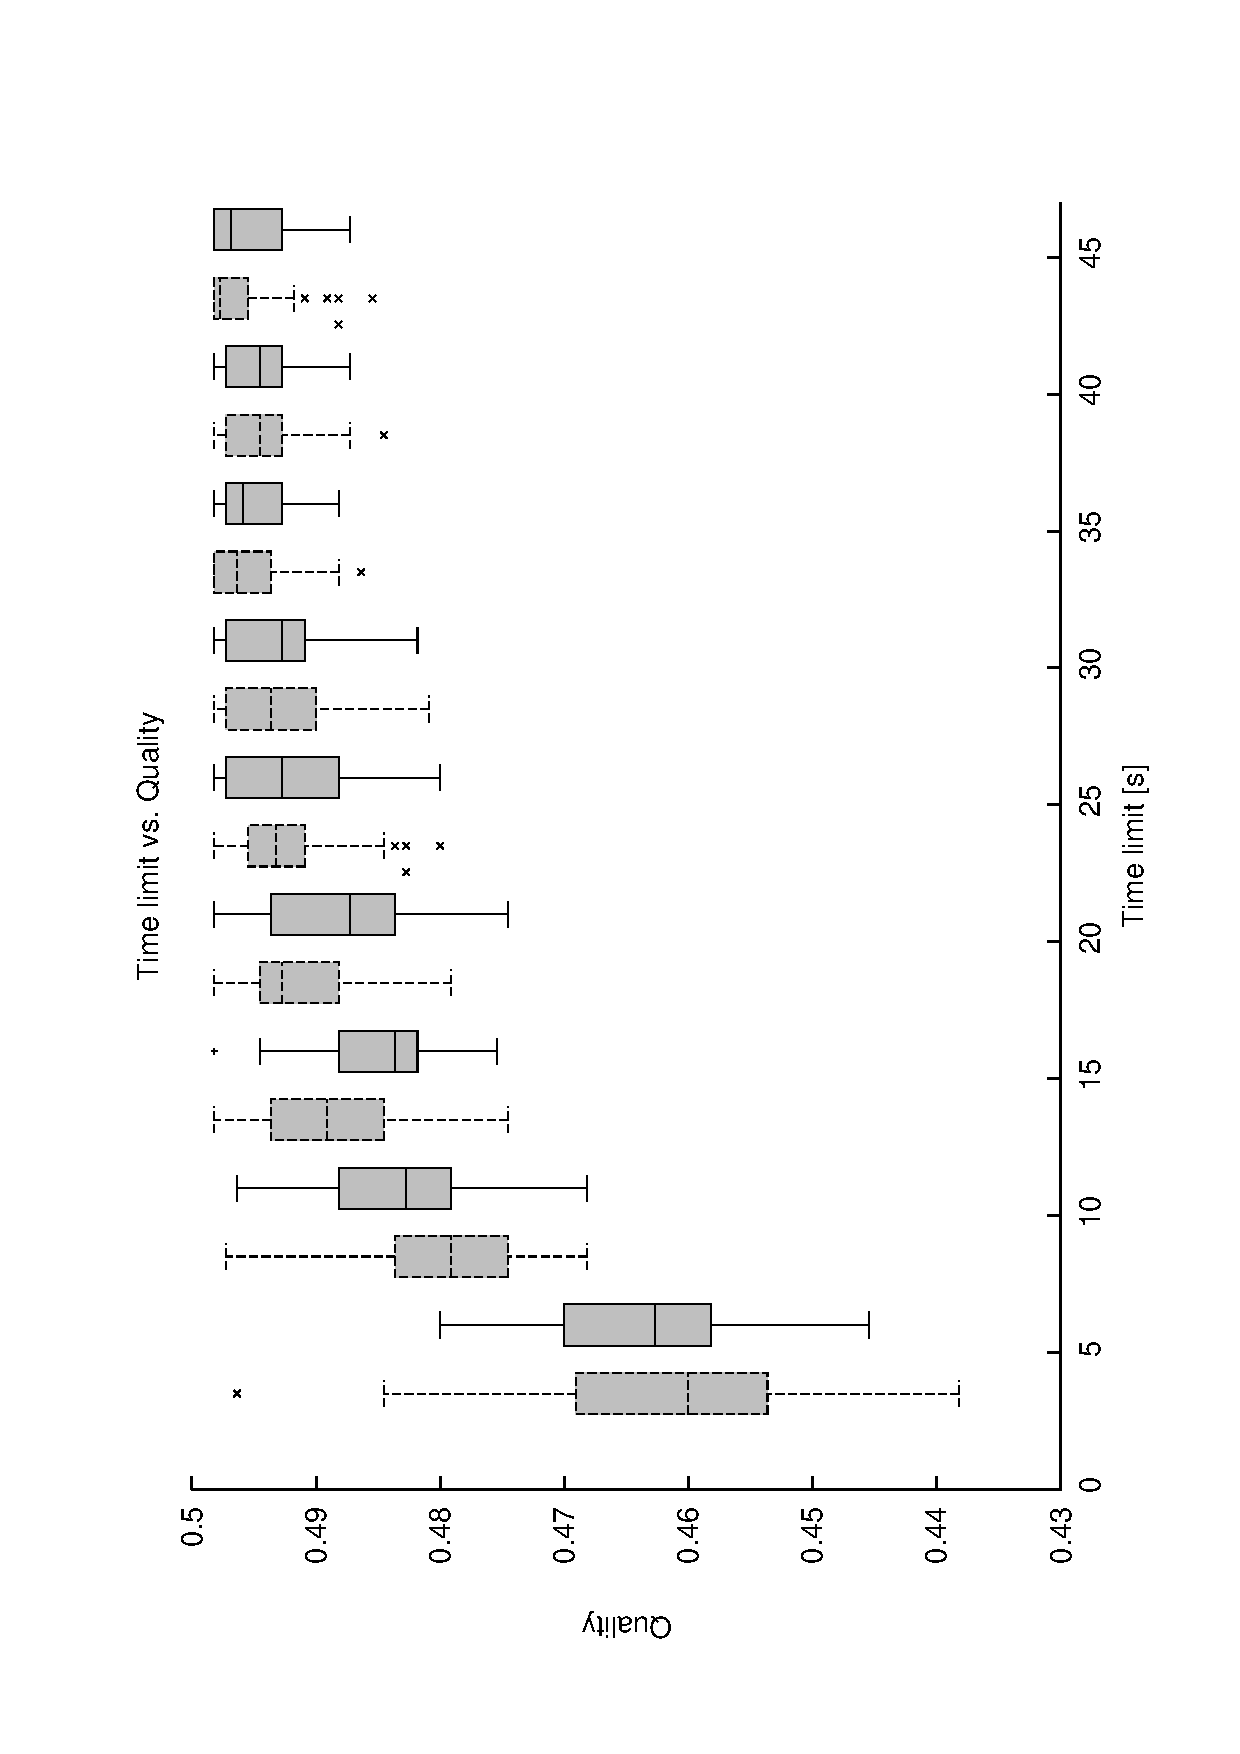
\includegraphics[width=\textwidth]{images/experiments/time-vs-quality}
\end{figure}

Results are in Figure \ref{image-experiment-time-vs-quality}. They should be interpreted as follows: for each time limit from 1 to 46 seconds there are two boxplots next to each other, the left, dashed one is the native GLPK, the right, solid one is the Cygwin GLPK. This is reflected in the tics on the X (time) axis, meaning that the axis cannot be interpreted in the usual way.

We can see from the graph that even though for smaller times (1 and 6 seconds, respectively) the Cygwin GLPK is reaching better qualities with smaller variance, starting from 11 seconds the native GLPK is at least as good or better for every following time. The results are inconclusive though, it is necessary to wait for confirmation from the second part of this experiment.

\begin{center}
\bigskip
\begin{tabular}{| l | l |}
  \hline
  \hline
  Input data        & all sized test data sets \\
  Iterations        & 50 \\
  Pool size         & 1 \\
  $\alpha$, $\beta$ & $1$, $1$ \\
  CH                & \heu{Glpk} \\
  IHs               & $\emptyset$ \\
  \hline
\end{tabular}
\bigskip
\end{center}

The other way to compare the performance of these two GLPK versions is to see how long it takes them to find the optimum for a set of data of increasing size. This experimental set will contain 550 configurations for each version. Every configuration will let \heu{Glpk} CH run for unlimited time, until it finds the optimum. This will be repeated in 50 iterations for each of the 11 files from the sized test data set (see Listing \ref{listing-experiment-glpk-native-vs-cygwin-2}). There will again be no IH, the only data we will collect are the times of the CH run in each case.\\

\begin{algorithm}
\caption{GLPK: native vs. Cygwin set generation 2}
\label{listing-experiment-glpk-native-vs-cygwin-2}
\begin{algorithmic}
\ENSURE experimental set $ES$
\STATE $ES \gets \emptyset$
\FOR{$i = 1 \to 50$}
	\FOR{$file \in $ sized test data}
    \STATE $ES \gets ES \cup \{file, CH = \heu{Glpk}(no\:limit), IH = \emptyset\}$
  \ENDFOR
\ENDFOR
\RETURN $ES$
\end{algorithmic}
\end{algorithm}

\begin{figure}
  \caption{Time Until Optimum}
  \label{image-experiment-time-until-optimum}
  \centering
    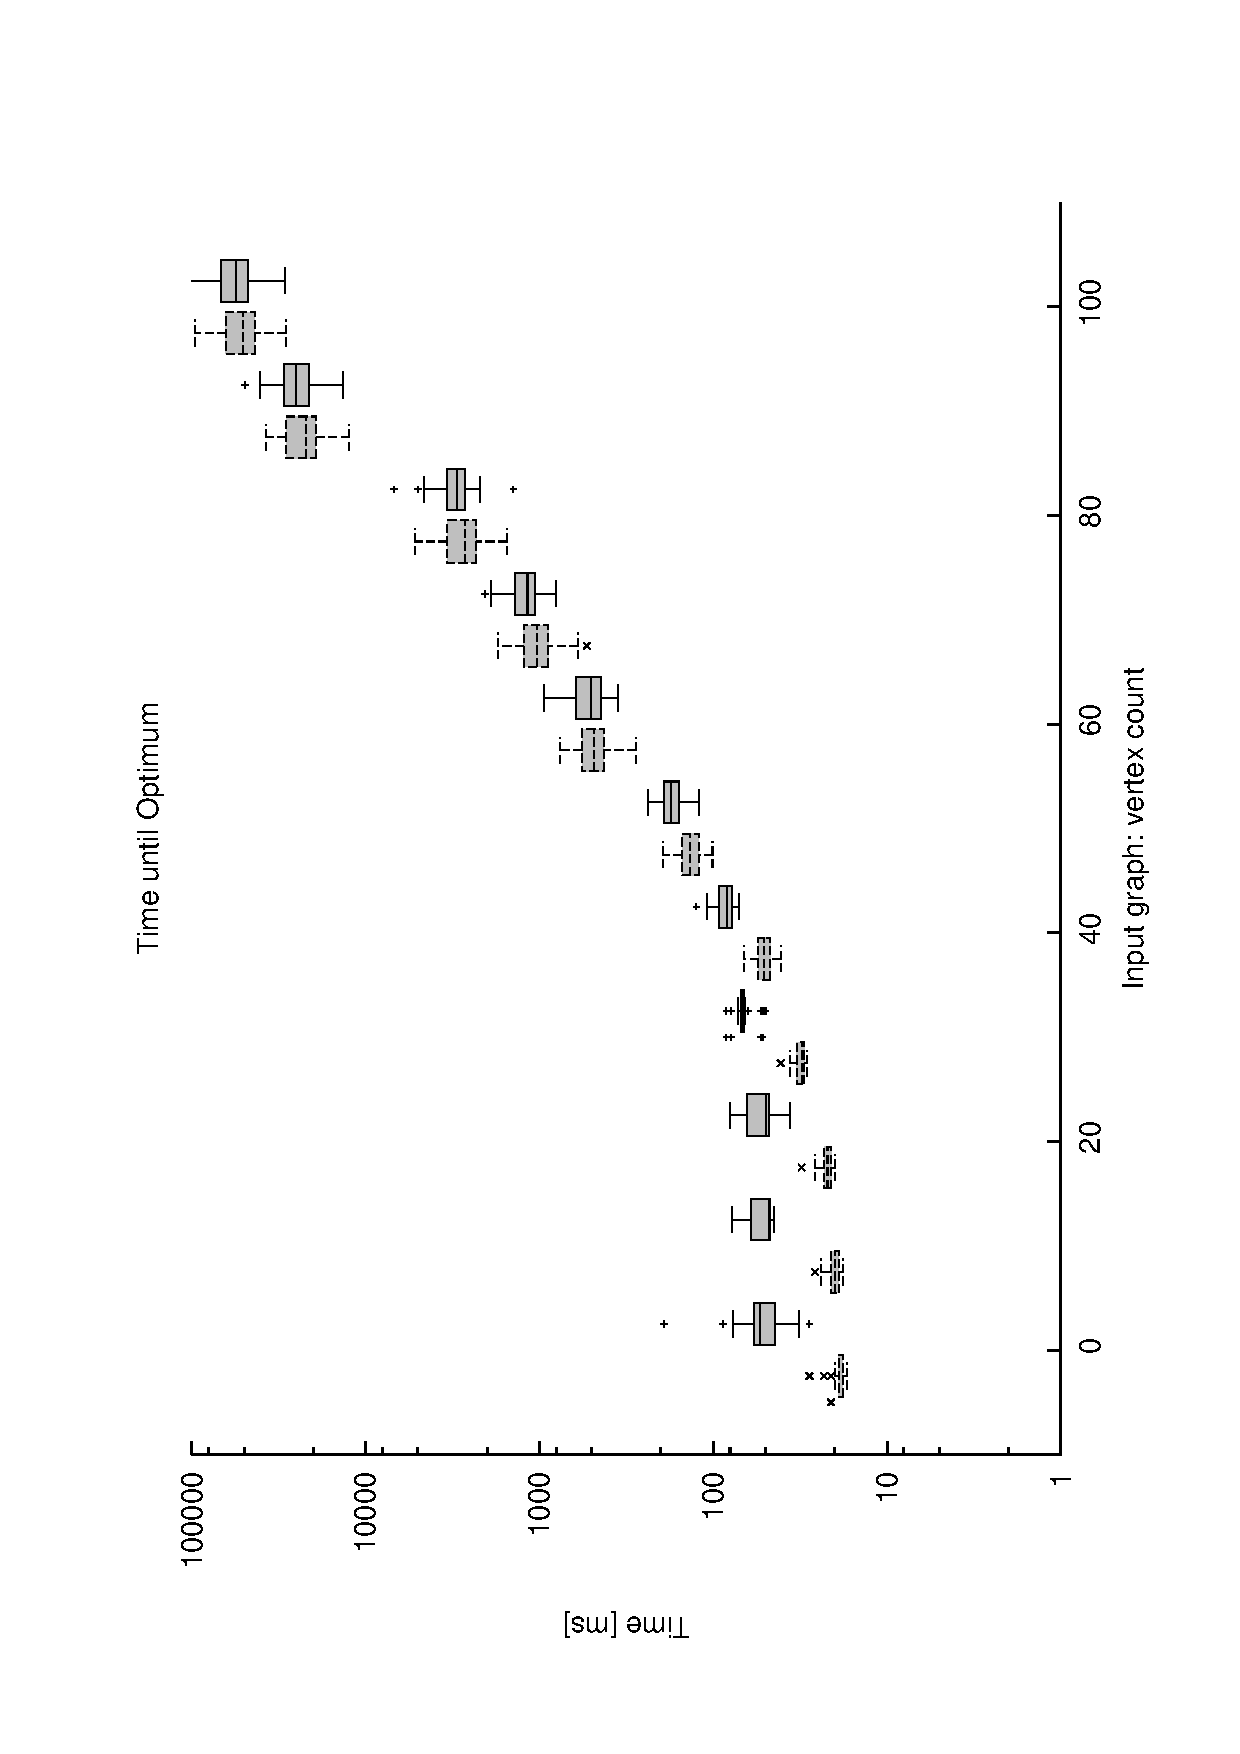
\includegraphics[width=\textwidth]{images/experiments/time-till-optimum}
\end{figure}

Results are in Figure \ref{image-experiment-time-until-optimum}, please take a note that the Y axis is in log scale. As with the previous case, the X axis cannot be interpreted in the usual way. For each data set there are two boxplots next to each other: the left one is the native GLPK, the right one is the Cygwin GLPK.

From these results it becomes clear that the native GLPK has in general shorter running times for each and every input data set than its Cygwin counterpart. This becomes less extreme with the increasing input size, which leads us to suspicion that the core parts of computation in both cases are equally powerful. Regardless of that, we shall be using the \textbf{native} GLPK for following experiments.

To conclude the first timing experiments we introduce a summary pie chart in Figure \ref{image-experiment-timing-summary}. This shows the typical distribution of times needed to find the optimum for the \dataset{OVA3} data set.

These experiments proved that for bigger data sets the times to reach the optimum might become too long. We shall attempt to find heuristics to reach the optimum faster in the following experiments.

% TODO fix this chart
\begin{figure}
  \caption{Timing Summary}
  \label{image-experiment-timing-summary}
  \centering
    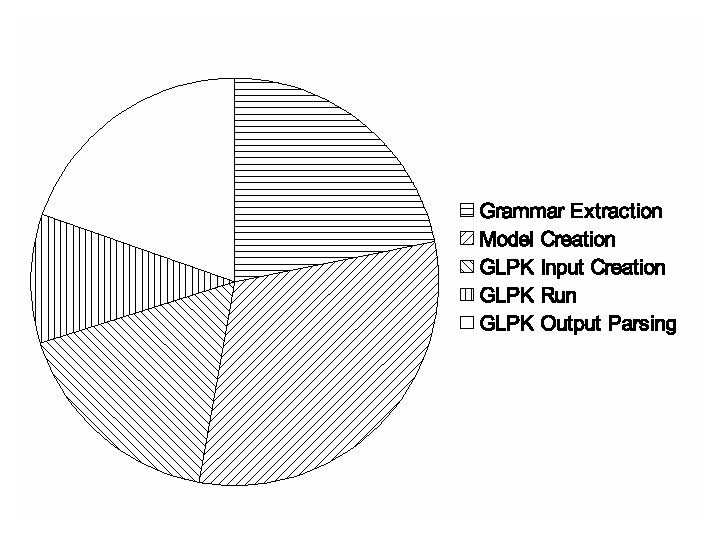
\includegraphics[width=.6\textwidth]{images/experiments/timing-pie}
\end{figure}

\subsection{\heu{Random} vs. \heu{Fuzzy} vs. \heu{FIDAX}}
\label{section-experiments-random-fuzzy-fidax}

%         NB class RandomVsFuzzyVsFidaxStart

Our investigation into various CHs will start by comparing \heu{FIDAX} from the original article \cite{fidax} to 2 of our trivial randomized hungry heuristics, \heu{Random} and \heu{Fuzzy}.

\begin{center}
\bigskip
\begin{tabular}{| l | l |}
  \hline
  \hline
  Input data set    & all official test data sets \\
  Iterations        & 50 \\
  Pool size         & 10 \\
  $\alpha$, $\beta$ & $1$, $1$ \\
  CH                & \heu{Random}, \heu{Fuzzy}, \heu{FIDAX} \\
  IHs               & $\emptyset$ \\
  \hline
\end{tabular}
\bigskip
\end{center}

The experimental set will contain 1650 configurations in total: 3 different CHs * 11 official test data sets * 50 iterations. There will be no improvement heuristics. The pool size will be set to 10, even though \heu{FIDAX} cannot not profit from this. Listing for this can be found in \ref{listing-experiment-random-fuzzy-fidax}.

We will be gathering the running time of the CH itself and quality of the best solution found for GnuPlot.\\

\begin{algorithm}
\caption{\heu{Random} vs. \heu{Fuzzy} vs. \heu{FIDAX} Set Generation}
\label{listing-experiment-random-fuzzy-fidax}
\begin{algorithmic}
\ENSURE experimental set $ES$
\STATE $ES \gets \emptyset$
\FOR{$i = 1 \to 50$}
	\FOR{$file \in $ official test data}
    \STATE $ES \gets ES \cup \{file, CH = \heu{Random}(pool = 10), IH = \emptyset\} \cup \{file, CH = \heu{Fuzzy}(pool = 10), IH = \emptyset\} \cup \{file, CH = \heu{FIDAX}, IH = \emptyset\}$
  \ENDFOR
\ENDFOR
\RETURN $ES$
\end{algorithmic}
\end{algorithm}

\begin{figure}
  \caption{Random vs. Fuzzy vs. FIDAX - Quality}
  \label{image-experiment-random-fuzzy-fidax-quality}
  \centering
    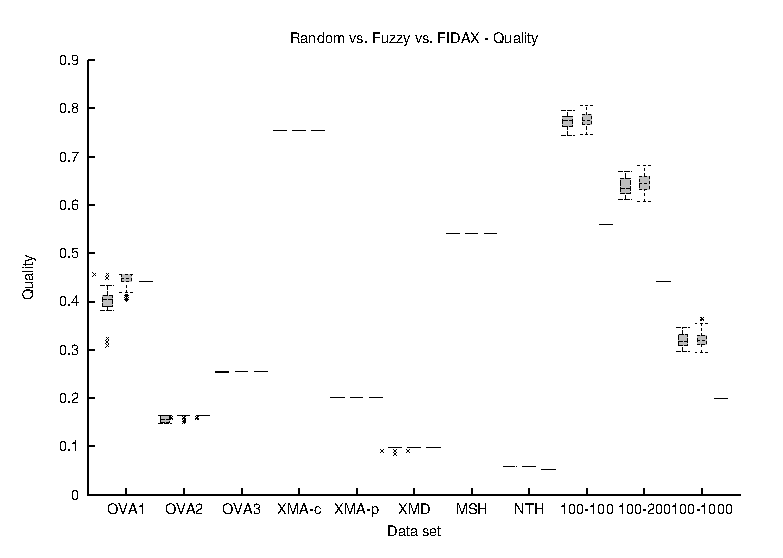
\includegraphics[width=\textwidth]{images/experiments/random-fuzzy-fidax-quality}
\end{figure}

\begin{figure}
  \caption{Random vs. Fuzzy vs. FIDAX - Time}
  \label{image-experiment-random-fuzzy-fidax-time}
  \centering
    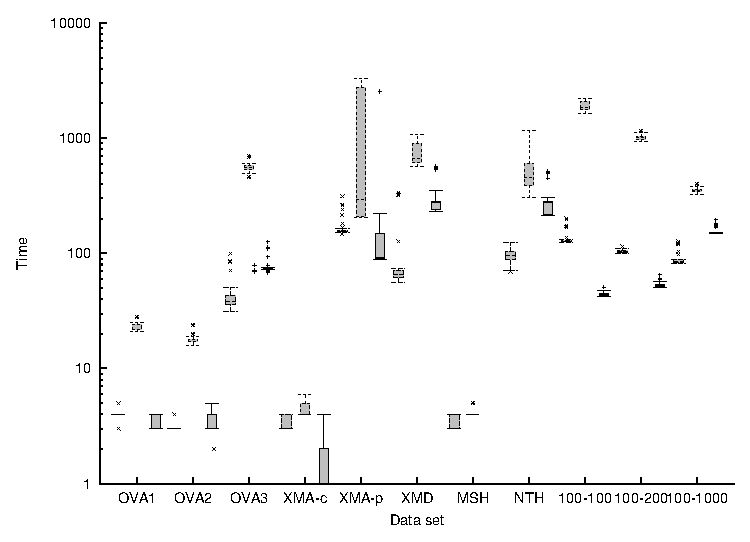
\includegraphics[width=\textwidth]{images/experiments/random-fuzzy-fidax-time}
\end{figure}

Results can be found in Figure \ref{image-experiment-random-fuzzy-fidax-quality} - qualities achieved and Figure \ref{image-experiment-random-fuzzy-fidax-time} - times spent. The Y (time) axis in the latter figure is again in log scale. For each data set there are 3 boxplots next to each other. The first, leftmost, represents \heu{Random}, second \heu{Fuzzy} and finally the third, rightmost is \heu{FIDAX}.

We can draw the following conclusions. \heu{Fuzzy} consistently finds the best solution, but it's by far the slowest of these CHs. The trivial \heu{Random} is better than \heu{FIDAX} in artificial as well as some real data.

\subsubsection{Improving \heu{FIDAX} with \heu{Hungry}}

%         NB class FidaxWithHungry

Now we shall try to answer a minor question, whether it is possible to improve \heu{FIDAX} by using \heu{Hungry} as IH. This short experiment answers that question.

\begin{center}
\bigskip
\begin{tabular}{| l | l |}
  \hline
  \hline
  Input data set    & all official test data sets \\
  Iterations        & 1 \\
  Pool size         & 1 \\
  $\alpha$, $\beta$ & $1$, $1$ \\
  CH                & \heu{FIDAX} \\
  IHs               & \heu{Hungry} or $\emptyset$ \\
  \hline
\end{tabular}
\bigskip
\end{center}

We need a pool size of one and only a single iteration - both \heu{FIDAX} and \heu{Hungry} are deterministic. We will try all official data sets, first with empty IH, second with \heu{Hungry} as IH. We will gather the qualities in each case and see whether there is any improvement.\\

The experimental results are summarized in the Table \ref{table-experiments-fidax-and-hungry} and are quite surprising. As trivial a heuristic \heu{Hungry} is, it is still able to improve the ID set found by \heu{FIDAX} by as much as almost 50\% (the last row, \dataset{100-1000}).

Table \ref{table-experiments-fidax-and-hungry-idsets} lists the ID attributes found in both cases for this most extreme input, \dataset{100-1000}. Note that the content of each cell means ``attribute \texttt{attr} in element \texttt{vertexXY} should be marked as ID attribute".

\begin{table}
  \caption{Results of adding \heu{Hungry} after \heu{FIDAX}}
  \bigskip
  \label{table-experiments-fidax-and-hungry}
  \centering
  \begin{tabular}{l | l | l}
    Data set & Quality - \heu{FIDAX} & Quality - \heu{FIDAX} + \heu{Hungry} \\
    \hline
    \dataset{OVA1}     & 0.4411764705882353  & 0.4411764705882353   \\
    \dataset{OVA2}     & 0.16346153846153846 & 0.16346153846153846  \\
    \dataset{OVA3}     & 0.25482414123443264 & \textbf{0.2553715615163541}   \\
    \dataset{XMA-c}    & 0.7546666666666666	 & 0.7546666666666666   \\
    \dataset{XMA-p}    & 0.2019306150568969	 & 0.2019306150568969   \\
    \dataset{XMD}      & 0.09786094165493509 & 0.09786094165493509  \\
    \dataset{MSH}      & 0.5416472778036296	 & 0.5416472778036296   \\
    \dataset{NTH}      & 0.05259709474828076 & \textbf{0.057918595422124436} \\
    \dataset{100-100}  & 0.56	               & \textbf{0.6766666666666669}   \\
    \dataset{100-200}  & 0.44200000000000017 & \textbf{0.5980000000000003}   \\
    \dataset{100-1000} & 0.19952380952380955 & \textbf{0.29619047619047617}  \\
  \end{tabular}
\end{table}

% TODO for some reason \texttt{\textbf{vertex5}} looks only like \texttt{vertex5}
\begin{table}
  \caption{ID Sets in \heu{FIDAX} Versus \heu{FIDAX} + \heu{Hungry}}
  \bigskip
  \label{table-experiments-fidax-and-hungry-idsets}
  \centering
  \begin{tabular}{l | l}
  \heu{FIDAX} & \heu{FIDAX} + \heu{Hungry} \\
  \hline
                    & \texttt{\textbf{vertex5}}  \\
                    & \texttt{\textbf{vertex26}} \\
  \texttt{vertex30} & \texttt{vertex30} \\
  \texttt{vertex31} & \texttt{vertex31} \\
  \texttt{vertex32} & \texttt{vertex32} \\
  \texttt{vertex34} & \texttt{vertex34} \\
  \texttt{vertex35} & \texttt{vertex35} \\
  \texttt{vertex36} & \texttt{vertex36} \\
  \texttt{vertex37} & \texttt{vertex37} \\
  \texttt{vertex39} & \texttt{vertex39} \\
                    & \texttt{\textbf{vertex60}} \\
                    & \texttt{\textbf{vertex69}} \\
                    & \texttt{\textbf{vertex70}} \\
  \texttt{vertex74} & \texttt{vertex74} \\
  \texttt{vertex75} & \texttt{vertex75} \\
  \texttt{vertex80} & \texttt{vertex80} \\
  \end{tabular}
\end{table}

\subsection{Best Standalone CH}

%         NB class BestStandaloneCH

% TODO re-run on Dual Core!

We shall now try to find the best standalone CH, that is the CH that finds on average the best solutions when run without any IHs. We need to set a time limit for \heu{Glpk} to make it an instance of \heu{Truncated Branch \& Bound}, and we shall use 1 second. This is the smallest time limit possible for GLPK and it is still a reasonably short time, fair to other CHs.

\begin{center}
\bigskip
\begin{tabular}{| l | l |}
  \hline
  \hline
  Input data        & all official test data sets \\
  Iterations        & 50 \\
  Pool size         & 10 \\
  $\alpha$, $\beta$ & $1$, $1$ \\
  CH                & various \\
  IHs               & $\emptyset$ \\
  \hline
\end{tabular}
\bigskip
\end{center}

We will use all the official data sets, set the pool size to 10 where applicable, $\alpha$ and $\beta$ to 1. This experiment will consist of 50 iterations * 11 data sets * 6 CHs = 3300 experimental configurations. See the Listing \ref{listing-experiment-best-standalone-ch} for details. This time we are not interested in run times, only in qualities which we shall gather in a format for GnuPlot.\\

\begin{algorithm}
\caption{Best Standalone CH Set Generation}
\label{listing-experiment-best-standalone-ch}
\begin{algorithmic}
\ENSURE experimental set $ES$
\STATE $ES \gets \emptyset$
\FOR{$file \in $ official test data}
	\FOR{$i = 1 \to 50$}
    	\STATE $ES \gets ES \cup \{file, CH = \heu{Random}, IH = \emptyset\}$
    	\STATE $ES \gets ES \cup \{file, CH = \heu{Fuzzy}, IH = \emptyset\}$
    	\STATE $ES \gets ES \cup \{file, CH = \heu{Incremental}, IH = \emptyset\}$
    	\STATE $ES \gets ES \cup \{file, CH = \heu{Removal}, IH = \emptyset\}$
    	\STATE $ES \gets ES \cup \{file, CH = \heu{FIDAX}, IH = \emptyset\}$
    	\STATE $ES \gets ES \cup \{file, CH = \heu{Glpk}(limit = 1), IH = \emptyset\}$
  \ENDFOR
\ENDFOR
\RETURN $ES$
\end{algorithmic}
\end{algorithm}

For data sets \heu{XMA-c}, \heu{XMA-p}, \heu{MSH} and \heu{NTH} every CH found the optimum every time. Graphs representing the results for remaining data sets can be found in Figure \ref{image-experiments-best-standalone-ch}.

\begin{figure}
  \caption{Best Standalone CH}
  \label{image-experiments-best-standalone-ch}
  \centering
  	\subfigure[\dataset{OVA1}]{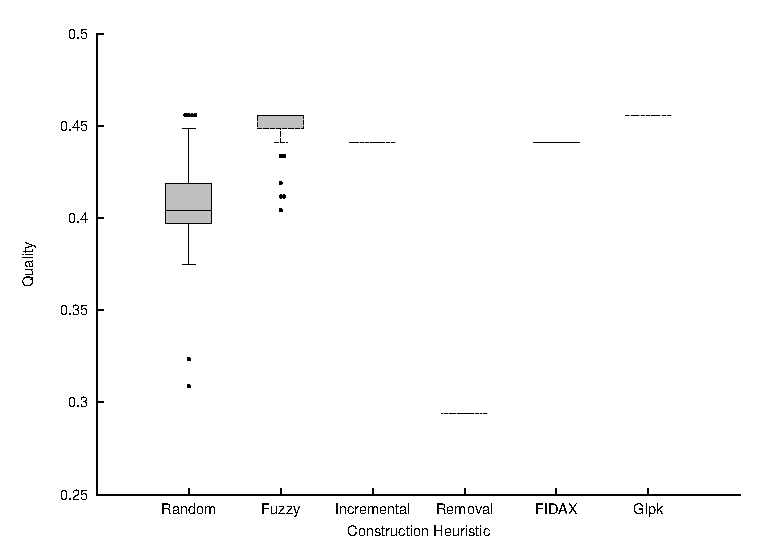
\includegraphics[width=.45\textwidth]{images/experiments/best-ch-OVA1}}
  	\subfigure[\dataset{OVA2}]{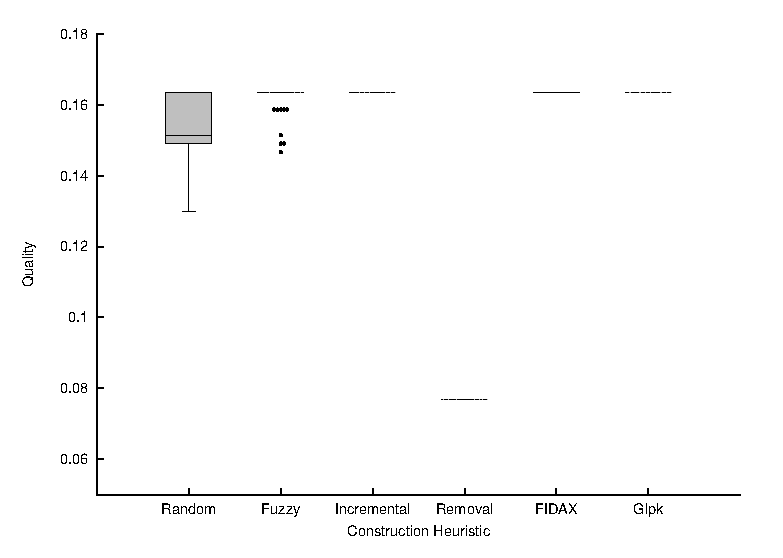
\includegraphics[width=.45\textwidth]{images/experiments/best-ch-OVA2}}
  	\subfigure[\dataset{OVA3}]{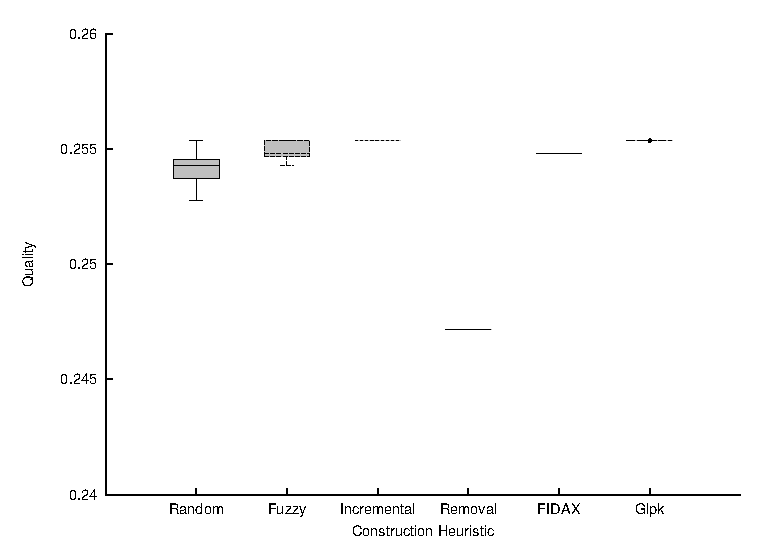
\includegraphics[width=.45\textwidth]{images/experiments/best-ch-OVA3}}
  	\subfigure[\dataset{XMD}]{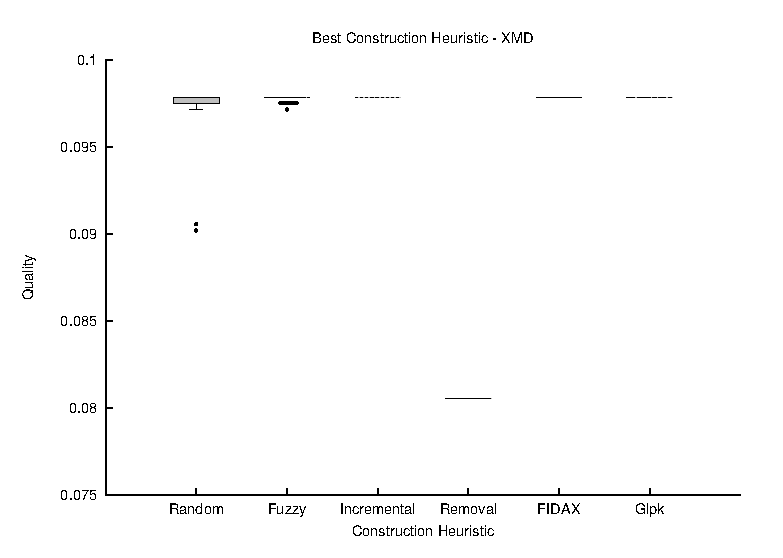
\includegraphics[width=.45\textwidth]{images/experiments/best-ch-XMD}}
   	\subfigure[\dataset{100-100}]{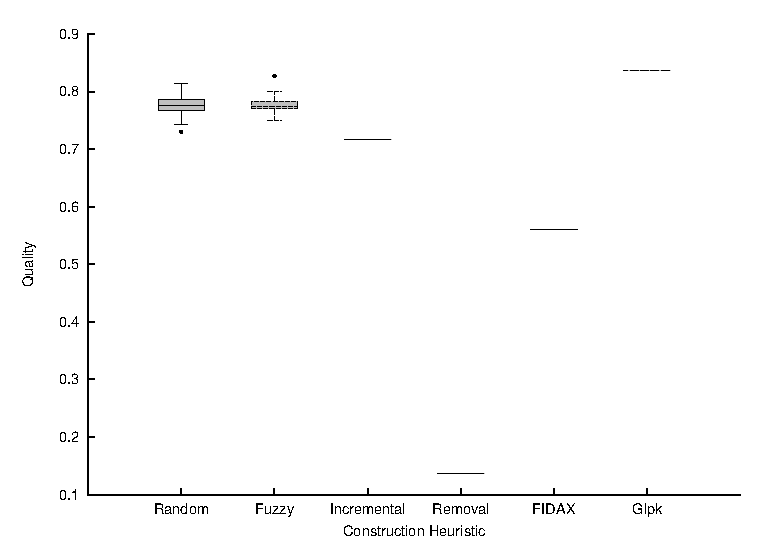
\includegraphics[width=.45\textwidth]{images/experiments/best-ch-100-100}}
  	\subfigure[\dataset{100-200}]{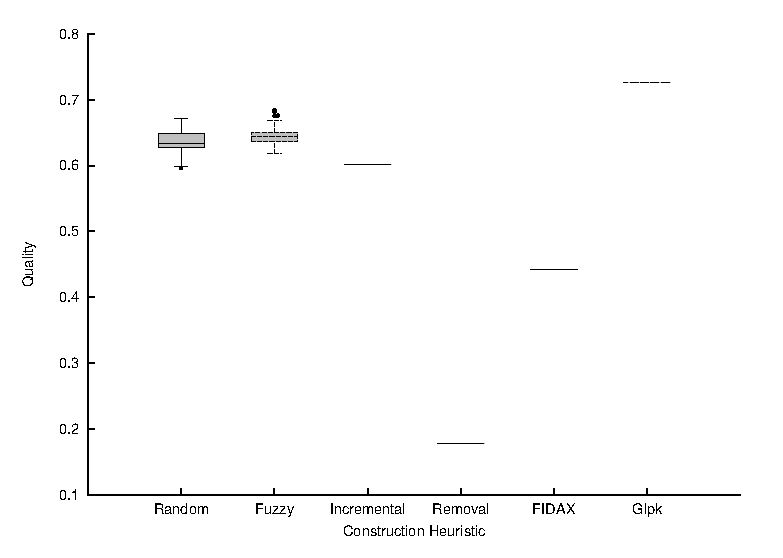
\includegraphics[width=.45\textwidth]{images/experiments/best-ch-100-200}}
  	\subfigure[\dataset{100-1000}]{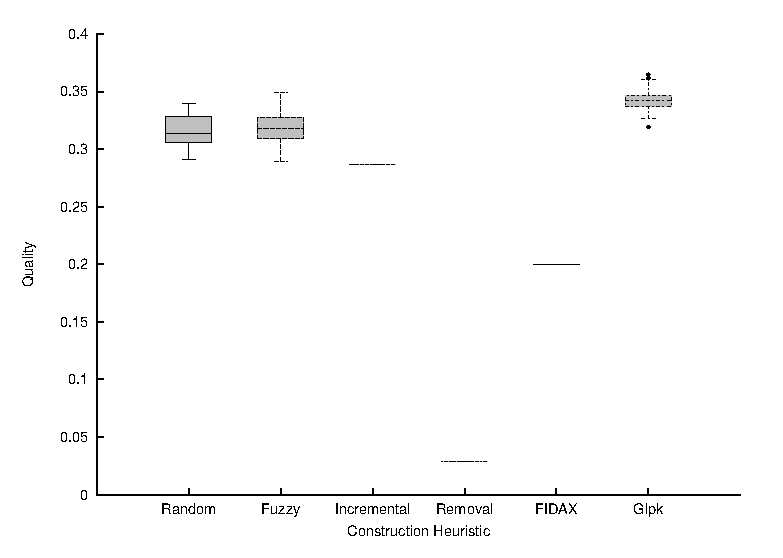
\includegraphics[width=.45\textwidth]{images/experiments/best-ch-100-1000}}
\end{figure}

We can see that \heu{Glpk} wins in every single case. We will start from there and try to build upon this result.

\subsection{Best IH for \heu{Glpk}}

%         NB class BestIHForGlpk

The next logical step will be to try to add one IH after the best CH we have found, \heu{Glpk}. We will investigate all IHs except for \heu{RandomRemove} and \heu{RemoveWorst}, which cannot help us at this time.

We should note that the combination \textit{best CH - best IH} found this way does not necessarily need to be the best one overall, because we find it using a hungry approach.

\begin{center}
\bigskip
\begin{tabular}{| l | l |}
  \hline
  \hline
  Input data        & \dataset{80-30}, \dataset{90-405}, \dataset{100-500}, \\
                    & \dataset{100-100}, \dataset{100-200}, \dataset{100-1000} \\
  Iterations        & 50 \\
  Pool size         & 10 \\
  $\alpha$, $\beta$ & $1$, $1$ \\
  CH                & \heu{Glpk} \\
  IHs               & \heu{Crossover}, \heu{Hungry}, \heu{Local Branching}, \heu{Mutation} \\
  \hline
\end{tabular}
\bigskip
\end{center}

This experimental set will contain 6 data sets * 50 iterations * 4 IHs = 1200 experimental configurations. Note that we are using only the most challenging data sets, as the combination of \heu{Glpk} as CH and any other IH is already an overkill for easier data sets.\\

\begin{algorithm}
\caption{Best IH for \heu{Glpk} Set Generation}
\label{listing-experiment-best-ih-for-glpk}
\begin{algorithmic}
\ENSURE experimental set $ES$
\STATE $ES \gets \emptyset$
\FOR{$file \in \{\dataset{80-30}, \dataset{90-405}, \dataset{100-500}, \dataset{100-100}, \dataset{100-200}, \dataset{100-1000}\}$}
	\FOR{$i = 1 \to 50$}
    	\STATE $ES \gets ES \cup \{file, CH = \heu{Glpk}(limit = 1), IH = \heu{Crossover}(ratio = 0.1, limit = 1)\}$
    	\STATE $ES \gets ES \cup \{file, CH = \heu{Glpk}(limit = 1), IH = \heu{Hungry}\}$
    	\STATE $ES \gets ES \cup \{file, CH = \heu{Glpk}(limit = 1), IH = \heu{Local Branching}(ratio = 0.1, limit = 1)\}$
    	\STATE $ES \gets ES \cup \{file, CH = \heu{Glpk}(limit = 1), IH = \heu{Mutation}(ratio = 0.1, limit = 1)\}$
  \ENDFOR
\ENDFOR
\RETURN $ES$
\end{algorithmic}
\end{algorithm}

The results are listed in Table \ref{table-experiments-best-ih-for-glpk}. We shall denote \textit{improvement} the absolute increase in quality after running \heu{Glpk} and after running the IH. The table now lists for each data set and each IH the average improvement as well as the standard deviation of the improvement. Bold number represents the best IH for that specific data set. \heu{Mutation} proves to be the best IH for 3 out of 6 data sets.

\begin{table}
  \caption{Best IH for \heu{Glpk}}
  \bigskip
  \label{table-experiments-best-ih-for-glpk}
  \centering
  \begin{tabular}{l || l | l || l | l}
             & \heu{Hungry} & \heu{Hungry} & \heu{Crossover} & \heu{Crossover} \\
    Data set & improv - avg & improv - stdev & improv - avg & improv - stdev \\
    \hline
    \dataset{80-320} & 0.00017 & 0.00118 & 0.00017 & 0.00118 \\
    \dataset{90-405} & 0.00502 & 0.00618 & 0.00033 & 0.00165 \\
    \dataset{100-500} & 0.00664 & 0.00667 & 0.00016 & 0.00081 \\
    \hline
    \dataset{100-100} & 0.00000 & 0.00000 & 0.00000 & 0.00000 \\
    \dataset{100-200} & 0.00000 & 0.00000 & 0.00000 & 0.00000 \\
    \dataset{100-1000} & 0.01630 & 0.01294 & 0.00180 & 0.00506 \\
  \end{tabular}    
	% TODO separate somehow
  \begin{tabular}{l || l | l || l | l}
             & \heu{LB} & \heu{LB} & \heu{Mutation} & \heu{Mutation} \\
    Data set & improv - avg & improv - stdev & improv - avg & improv - stdev \\
    \hline
    \dataset{80-320} & \textbf{0.00072} & 0.00223 & 0.00064 & 0.00218 \\
    \dataset{90-405} & 0.00698 & 0.00616 & \textbf{0.00851} & 0.00659 \\
    \dataset{100-500} & 0.00796 & 0.00797 & \textbf{0.00964} & 0.00804 \\
    \hline
    \dataset{100-100} & 0.00000 & 0.00000 & 0.00000 & 0.00000 \\
    \dataset{100-200} & 0.00000 & 0.00000 & 0.00000 & 0.00000 \\
    \dataset{100-1000} & 0.01710 & 0.01188 & \textbf{0.02337} & 0.01558 \\
  \end{tabular}
\end{table}

\subsubsection{\heu{Random} as CH}

%         NB class CHForMutation

As we mentioned before, we chose the combination \heu{Glpk} and \heu{Mutation} in a hungry manner. We will now try to take a step back and attempt to replace \heu{Glpk} with \heu{Random}, hoping to get similar qualities in much shorter time (a reminder: \heu{Glpk} always takes 1 second).

\begin{center}
\bigskip
\begin{tabular}{| l | l |}
  \hline
  \hline
  Input data        & \dataset{80-30}, \dataset{90-405}, \dataset{100-500}, \\
                    & \dataset{100-100}, \dataset{100-200}, \dataset{100-1000} \\
  Iterations        & 50 \\
  Pool size         & 10 \\
  $\alpha$, $\beta$ & $1$, $1$ \\
  CH                & \heu{Random} or \heu{Glpk} \\
  IHs               & \heu{Mutation} \\
  \hline
\end{tabular}
\bigskip
\end{center}

Setup used will be almost identical to that from the previous experiment. Experimental set will consist of 6 data sets * 50 iterations * 2 CHs = 600 experimental configurations, see Listing \ref{listing-experiment-ch-for-mutation}. We shall collect the eventual quality after running both the CH and the IH in format suited for GnuPlot.\\

\begin{algorithm}
\caption{\heu{Random} as CH Set Generation}
\label{listing-experiment-ch-for-mutation}
\begin{algorithmic}
\ENSURE experimental set $ES$
\STATE $ES \gets \emptyset$
\FOR{$file \in \{\dataset{80-30}, \dataset{90-405}, \dataset{100-500}, \dataset{100-100}, \dataset{100-200}, \dataset{100-1000}\}$}
	\FOR{$i = 1 \to 50$}
    	\STATE $ES \gets ES \cup \{file, CH = \heu{Random}, IH = \heu{Mutation}(ratio = 0.1, limit = 1)\}$
    	\STATE $ES \gets ES \cup \{file, CH = \heu{Glpk}(limit = 1), IH = \heu{Mutation}(ratio = 0.1, limit = 1)\}$
  \ENDFOR
\ENDFOR
\RETURN $ES$
\end{algorithmic}
\end{algorithm}

Results are summarized in Figure \ref{image-experiment-ch-for-mutation}. Again, for each data set there are two boxplots representing \heu{Random} (left one) and \heu{Glpk} (right one). The combination \heu{Glpk} + \heu{Mutation} always finds the optimum for the simpler data sets, thus the collapsed boxplots. Moreover, it achieves higher quality in each data set. On the other hand, combination \heu{Random} + \heu{Mutation} has much shorter running times and in the biggest (and hardest) data set \dataset{100-1000} has almost comparable results. This makes it a reasonable choice for big inputs where short time is more important than optimal quality.

\begin{figure}
  \caption{CH for \heu{Mutation}}
  \label{image-experiment-ch-for-mutation}
  \centering
    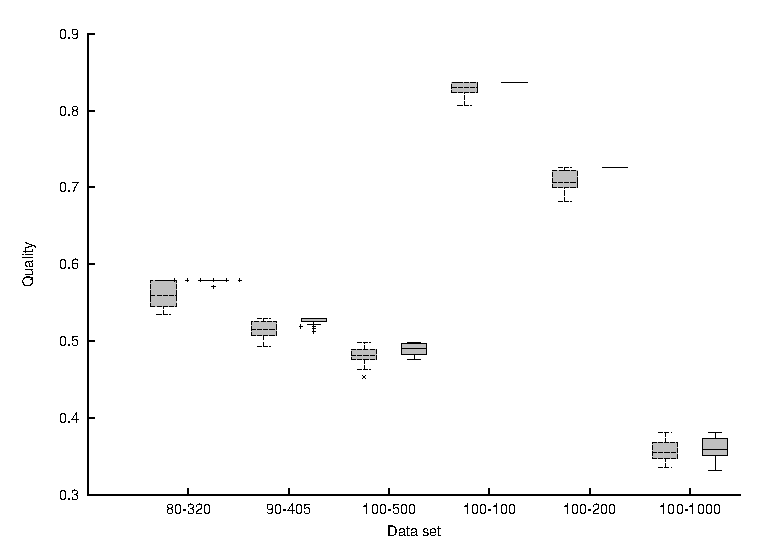
\includegraphics[width=\textwidth]{images/experiments/ch-for-mutation}
\end{figure}

% TODO this subsection does not play well with the ToC - how to put something else in the ToC than is here?
\subsection{Various $\alpha$, $\beta$}

After finding the best combination of a CH and IH we turn our attention to some of the parameters. The first ones are the $\alpha$ and $\beta$ from the definition of our weight function. % TODO link
A short reminder: the weight is defined as TODO copy formula. It is thus obvious that only the \textit{ratio} between $\alpha$ and $\beta$ matters, not their actual values. This means that investigating effects of these parameters is in fact a 1-dimensional problem. However, for simplicity's sake we will use 25 combinations of various $\alpha$ and $\beta$ and normalize them only during evaluation.

It is worthy noting that we do not expect any changes in performance of heuristics and we will limit the inquiry to different ID sets produced under different settings.

\begin{center}
\bigskip
\begin{tabular}{| l | l |}
  \hline
  \hline
  Input data        & realistic + converted official test data sets \\
  Iterations        & 1 \\
  Pool size         & 1 \\
  $\alpha$, $\beta$ & $\{0.1, 0.25, 0.5, 0.75, 1\} \times \{0.1, 0.25, 0.5, 0.75, 1\}$ \\ % TODO this is not the best way to write it
  CH                & \heu{Glpk} \\
  IHs               & $\emptyset$ \\
  \hline
\end{tabular}
\bigskip
\end{center}

This experimental set will contain 5 different $\alpha$ settings * 5 $\beta$ settings * 8 data sets = 200 experimental configurations. We are not using the artificial data sets, because the way they are generated (attribute values are random numbers) they cannot possibly create different optimal ID sets. The pseudocode capturing this is in Listing \ref{listing-experiment-various-betas}. We will use \heu{Glpk} constrained to 1 second (thus making it an instance of \heu{Truncated Branch \& Bound}) and no IHs. Pool size as well as iteration count will be 1. We are noting the actual ID set found by the run of the heuristic.\\

\begin{algorithm}
\caption{Various Values of $\alpha$ and $\beta$ Set Generation}
\label{listing-experiment-various-betas}
\begin{algorithmic}
\ENSURE experimental set $ES$
\STATE $ES \gets \emptyset$
\FOR{$\alpha \in \{0.1, 0.25, 0.5, 0.75, 1\}$}
  \FOR{$\beta \in \{0.1, 0.25, 0.5, 0.75, 1\}$}
    \FOR{$file \in $ realistic of converted official test data}
    	\STATE $ES \gets ES \cup \{file, CH = \heu{Glpk}(limit = 1, alpha = \alpha, beta = \beta), IH = \emptyset\}$
    \ENDFOR
  \ENDFOR
\ENDFOR
\RETURN $ES$
\end{algorithmic}
\end{algorithm}

Following data sets have the same optimal ID sets regardless of the setting of $\alpha$ and $\beta$: \dataset{MSH}, \dataset{NTH}, \dataset{XMA-c}, \dataset{XMA-p}. The \dataset{OVA*} data sets showed various dependencies on $\alpha$ and $\beta$, we shall now describe one representative example.

\subsubsection{Results for \dataset{OVA1}}

The 2 different ID sets found for various $\alpha$ and $\beta$ in \dataset{OVA1} are listed in Table \ref{table-experiments-various-betas-ova1} (note that the actual names had to be anonymized for reasons discussed in Section \ref{section-realistic-data}). The differing attribute mapping is highlited.

\begin{table}
  \caption{Different ID Sets Found for \dataset{OVA1}}
  \bigskip
  \label{table-experiments-various-betas-ova1}
  \centering
  \begin{tabular}{c || c}
    ID set \textbf{1}: element@attribute & ID set \textbf{2}: element@attribute \\
    \hline
    \texttt{aff@fa} & \texttt{aff@fa} \\
    \texttt{com@ty} & \texttt{com@ty} \\
    \texttt{cre@da} & \texttt{cre@da} \\
    \texttt{cri@te} & \texttt{cri@te} \\
    \texttt{cve@st} & \texttt{cve@st} \\
    \texttt{\textbf{def@id}} & \texttt{\textbf{def@cl}} <- \\ % TODO again, my bold typewriter does not work
    \texttt{fil@co} & \texttt{fil@co} \\
    \texttt{mod@da} & \texttt{mod@da} \\
    \texttt{ova@xs} & \texttt{ova@xs} \\
    \texttt{pat@op} & \texttt{pat@op} \\
    \texttt{sof@op} & \texttt{sof@op} \\
    \texttt{sta@da} & \texttt{sta@da} \\
    \texttt{sub@or} & \texttt{sub@or} \\
    \texttt{sbt@te} & \texttt{sbt@te} \\
  \end{tabular}
\end{table}

Table \ref{table-experiments-various-betas-ova1-effect} summarizes the dependency of the ID set found on various values of $\alpha$, $\beta$. We than define the $\alpha-ratio$ as $ \dfrac{\alpha}{\alpha + \beta} $ and summarize the findings in a linear manner, sorted by increasing $\alpha-ratio$ in Table \ref{table-experiments-various-betas-ova1-ratio-effect}. Note that the $\alpha-ratio$s are not unique due to the way we constructed the experimental configurations here.

\begin{table}
  \caption{Effect of $\alpha$, $\beta$ on ID Set Found for \dataset{OVA1}}
  \bigskip
  \label{table-experiments-various-betas-ova1-effect}
  \centering
  \begin{tabular}{c | c  c  c  c  c}
    $\alpha$ \textbackslash $\beta$ & 0.1 & 0.25 & 0.5 & 0.75 & 1 \\
    \hline
    0.1  & 1 & 2 & 2 & 1 & 1 \\
    0.25 & 2 & 2 & 2 & 1 & 2 \\
    0.5  & 2 & 1 & 1 & 1 & 2 \\
    0.75 & 1 & 2 & 1 & 2 & 1 \\
    1    & 1 & 2 & 1 & 1 & 2 \\
  \end{tabular}
\end{table}

\begin{table}
  \caption{Effect of $\alpha-ratio$ on ID Set Found for \dataset{OVA1}}
  \bigskip
  \label{table-experiments-various-betas-ova1-ratio-effect}
  \centering
  \begin{tabular}{c | c || c |  c}
    $\alpha-ratio$ & ID set & $\alpha-ratio$ & ID set \\
    \hline
    0,091	& 1 & 0,500	& 2 \\
    0,118	& 1 & 0,500	& 2 \\
    0,167	& 2 & 0,571	& 1 \\
    0,200	& 2 & 0,600	& 1 \\
    0,250	& 1 & 0,667	& 1 \\
    0,286	& 2 & 0,667	& 1 \\
    0,333	& 2 & 0,714	& 2 \\
    0,333	& 2 & 0,750	& 2 \\
    0,400	& 1 & 0,800	& 2 \\
    0,429	& 1 & 0,833	& 2 \\
    0,500	& 1 & 0,882	& 1 \\
    0,500	& 2 & 0,909	& 1 \\
    0,500	& 1 &       &   \\
  \end{tabular}
\end{table}

Interestingly enough, there is no clear separation between the two ID sets depending on the $\alpha-ratio$ to be found. The very existence of the two sets might be due to the fact that \heu{Glpk} randomizes the order in which AMs are presented to the external GLPK solver. However, this question is outside of the scope of this work, and shall be left for future work.

\subsection{Ignoring Text Data}

%         NB class IgnoreTextData

When considering data sets such as \dataset{XMA-p}, we notice that they contain a lot of simple text nodes that do not contribute to our search, but possibly slow it down. Precisely for this reason the \jmodule{BasicIGG} module in jInfer contains an option to turn off processing of such nodes. (It also allows to ignore the content of attributes, but this would be devastating to our cause.) Ignoring the content of text nodes means internally that these are created, but their actual string content is skipped and not saved in the memory structures. This means that the whole data model occupies less space on the heap, which can possibly lead to better performance.

We shall now investigate this matter by taking the biggest data set \dataset{XMA-p} containing a lot of text data.

\begin{center}
\bigskip
\begin{tabular}{| l | l |}
  \hline
  \hline
  Input data        & \dataset{XMA-p} \\
  Iterations        & 50 \\
  Pool size         & 1 \\
  $\alpha$, $\beta$ & $1$, $1$ \\
  CH                & \heu{Glpk} \\
  IHs               & not applicable \\
  \hline
\end{tabular}
\bigskip
\end{center}

Our experimental set will contain 50 iterations * 2 = 100 experimental configurations as described in Listing \ref{listing-experiment-ignore-text-data}. We will be using \heu{Glpk} limited to 1 second with no additional IH and pool size set to 1. After the first 50 iterations we will turn on the option to ignore the simple text node data and run the same 50 iterations again. We will be collecting the grammar extraction (GE) and model creation (MC) times as in the experiment in Section \ref{section-grammar-model-timing}.\\

\begin{algorithm}
\caption{Ignoring Text Data Set Generation}
\label{listing-experiment-ignore-text-data}
\begin{algorithmic}
\ENSURE experimental set $ES$
\STATE $ES \gets \emptyset$
\FOR{$i \in 1 \to 50 $}
  \STATE $ES \gets ES \cup \{\dataset{XMA-p}, CH = \heu{Glpk}(limit = 1), IH = \emptyset\}$
\ENDFOR
\STATE \textbf{set} ``ignore text data"
\FOR{$i \in 1 \to 50 $}
  \STATE $ES \gets ES \cup \{\dataset{XMA-p}, CH = \heu{Glpk}(limit = 1), IH = \emptyset\}$
\ENDFOR
\RETURN $ES$
\end{algorithmic}
\end{algorithm}

Results are summarized in Figure \ref{image-experiment-ignore-text-data}. Boxplots drawn in dashed lines represent the original case, not ignoring the text data. Solid lines represent the case where we ignore the text data.

Interestingly, the grammar extraction times tend to be shorter in the case when text data is not ignored, although this is inconclusive. However, there is a clear improvement of about 50 \% in the case of model creation times. The conclusion then is to ignore the simple text node content whenever possible when finding ID attributes.

\begin{figure}
  \caption{Ignoring Text Data}
  \label{image-experiment-ignore-text-data}
  \centering
    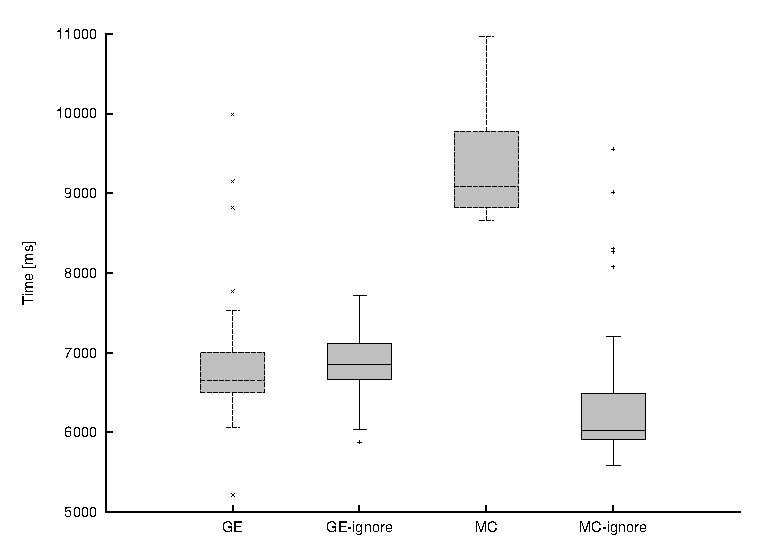
\includegraphics[width=\textwidth]{images/experiments/ignore-text-data}
\end{figure}

\subsection{Chaining the IHs}

%         NB class ChainedIHsX

In this section we will describe the most interesting experimental area, that is chaining more than one improvement heuristics and running them in a loop. Unfortunately, the sheer number of possible combinations in which IHs can be ordered (as well as the number of ways to set their parameters) prohibits us from investigating this in depth.

We shall then employ a higher-level heuristic: we will choose 3 strategies (lists of IHs, or metaheuristics), assess their performance to find the best one and then tune its parameters. This approach is by no means exhaustive, it is just a probe in the problem space.

The 3 strategies we will be assessing will be constructed from the following instances of improvement heuristics:

\begin{itemize}
	\item \heu{RR} is \heu{RandomRemove} with $ratio$ set to $0.1$.
	\item \heu{MUT} is \heu{Mutation} with $ratio$ set to $0.1$ and time limit set to 1 second.
	\item \heu{CX} is \heu{Crossover} with $ratio$ set to $0.1$ and time limit set to 1 second.
	\item \heu{LB} is \heu{LocalBranching} with $ratio$ set to $0.1$ and time limit set to 1 second.
	\item \heu{RW} is \heu{RemoveWorst}.
	\item \heu{H} is \heu{Hungry}.
\end{itemize}

The strategies themselves shall be the following:

\begin{itemize}
	\item \textit{\textbf{Strategy 1}}. \heu{RR} $\rightarrow$ \heu{MUT} $\rightarrow$ \heu{RR} $\rightarrow$ \heu{CX} $\rightarrow$ \heu{RW} $\rightarrow \ldots$
	\item \textit{\textbf{Strategy 2}}. \heu{CX} $\rightarrow$ \heu{RW} $\rightarrow$ \heu{MUT} $\rightarrow \ldots$
	\item \textit{\textbf{Strategy 3}}. \heu{CX} $\rightarrow$ \heu{RR} $\rightarrow$ \heu{MUT} $\rightarrow$ \heu{RW} $\rightarrow$ \heu{LB} $\rightarrow$ \heu{RW} $\rightarrow \ldots$
\end{itemize}

\begin{center}
\bigskip
\begin{tabular}{| l | l |}
  \hline
  \hline
  Input data        & all official test data sets \\
  Iterations        & 20 \\
  Pool size         & 10 \\
  $\alpha$, $\beta$ & $1$, $1$ \\
  CH                & \heu{Random} \\
  IHs               & various \\
  \hline
\end{tabular}
\bigskip
\end{center}

The experimental set will consist of 3 strategies * 11 data sets * 20 iterations = 660 experimental configurations. Their construction is formalized in the Listing \ref{listing-experiment-chaining-ihs}. The construction heuristic will be \heu{Random} with pool size 10. All the ratios are set to $0.1$ for the time being. The termination criterion is set to limit the total runtime to 10 seconds and (potentialy) infinite iterations.

Data gathered will be traces like the one in Appendix \ref{appendix-trace} - after each iteration, the time taken so far and the quality of incumbent solution is noted.\\

\begin{algorithm}
\caption{Chaining IHs Set Generation}
\label{listing-experiment-chaining-ihs}
\begin{algorithmic}
\ENSURE experimental set $ES$
\STATE $ES \gets \emptyset$
\STATE $\heu{MUT} \gets \heu{Mutation}(ratio = 0.1, limit = 1)$
\STATE $\heu{CX} \gets \heu{Crossover}(ratio = 0.1, limit = 1)$
\STATE $\heu{LB} \gets \heu{LocalBranching}(ratio = 0.1, limit = 1)$
\STATE $\heu{RR} \gets \heu{RandomRemove}(ratio = 0.1)$
\STATE $\heu{H} \gets \heu{Hungry}$
\STATE $\heu{RW} \gets \heu{RemoveWorst}$
\STATE $IHs \gets \emptyset$

\STATE $IHs \gets IHs \cup (\heu{RR}, \heu{MUT}, \heu{RR}, \heu{CX}, \heu{RW})$

\STATE $IHs \gets IHs \cup (\heu{CX}, \heu{RW}, \heu{MUT})$

\STATE $IHs \gets IHs \cup (\heu{CX}, \heu{RR}, \heu{MUT}, \heu{RW}, \heu{LB}, \heu{RW}, \heu{H})$

\FOR{$ih \in IHs$}
  \FOR{$file \in $ official test data}
    \FOR{$i = 1 \to 20$}
      \STATE $ES \gets ES \cup \{file, CH = \heu{Random}, IH = ih, limit = 10 seconds\}$
    \ENDFOR
  \ENDFOR
\ENDFOR
\RETURN $ES$
\end{algorithmic}
\end{algorithm}

Resulting traces for each data set can be summarized in graphs like the one for \heu{100-100} in Figure \ref{image-experiment-chained-ihs-s1}. This one deserves more explanation than usual.

\begin{figure}
  \caption{Chained IHs - \dataset{100-100} Results for Strategy 1}
  \label{image-experiment-chained-ihs-s1}
  \centering
    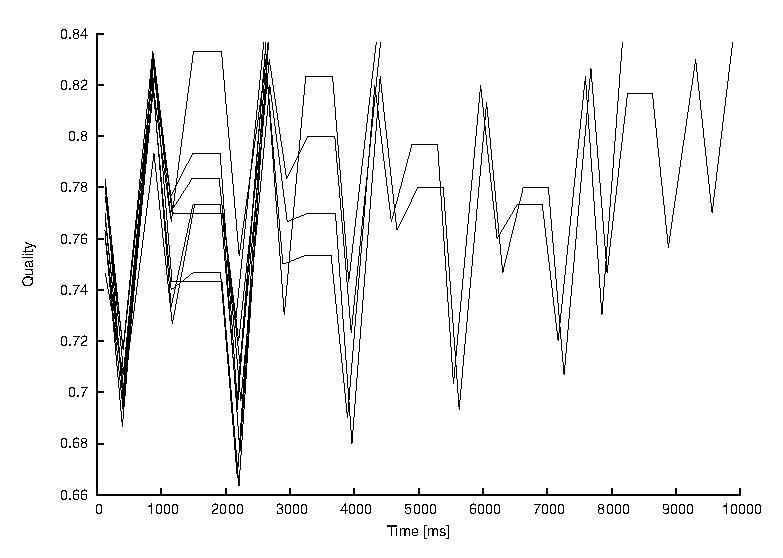
\includegraphics[width=\textwidth]{images/experiments/chained-ihs-s1}
\end{figure}

X and Y axes represent the time and quality, as usual. Each line represents one run of the strategy (metaheuristic) in the following way: the N\textsuperscript{th} break in the line (i.e. the N\textsuperscript{th} data point) is the partial result after the N\textsuperscript{th} step of the strategy. Its X position denotes the absolute time in which this step finished, and its Y position represents the incumbent solution quality after this step. Every time a line disappears before reaching 10 seconds it means that this metaheuristic run found the optimum before the 10 second mark. There is an obvious repetitive regularity in the shape of each line, this corresponds to the fact that there is a finite number of IHs in this strategy (5 of them in Strategy 1) which repeat over time. The obvious similarity between different lines corresponds to the fact that each run is from the same strategy, and over time, they do the same steps.

We can see effects of different IHs from this graph:
\begin{itemize}
	\item Every $(1 + 5k)$\textsuperscript{th} and $(3 + 5k)$\textsuperscript{th} step is a \heu{RandomRemove}, and each time this happens there is a rather sharp drop in quality
	\item Every $(2 + 5k)$\textsuperscript{th} step is a \heu{Mutation}, and there is a consistent increase in quality each time.
	\item Every $(4 + 5k)$\textsuperscript{th} step is a \heu{Crossover}, and each time it happens there is a consistent increase, yet smaller than with \heu{Mutation}.
	\item Every $5k$\textsuperscript{th} step is a \heu{RemoveWorst}, and as expected, this removes the worst solution not touching the best ones that decide the incumbent quality. The line thus stays flat every time it happens.
\end{itemize}

In this particular example there is only 1 run out of 10 that does not finish (find optimum) under the 10 second mark.\\

There are two more graphs like this in Figures \ref{image-experiment-chained-ihs-s2} and \ref{image-experiment-chained-ihs-s3} for comparison, capturing Strategy 2 and Strategy 3 respectively working on the same data set, \dataset{100-100}. Describing them in detail is unfortunately outside of the scope of this work.\\

\begin{figure}
  \caption{Chained IHs - \dataset{100-100} Results for Strategy 2}
  \label{image-experiment-chained-ihs-s2}
  \centering
    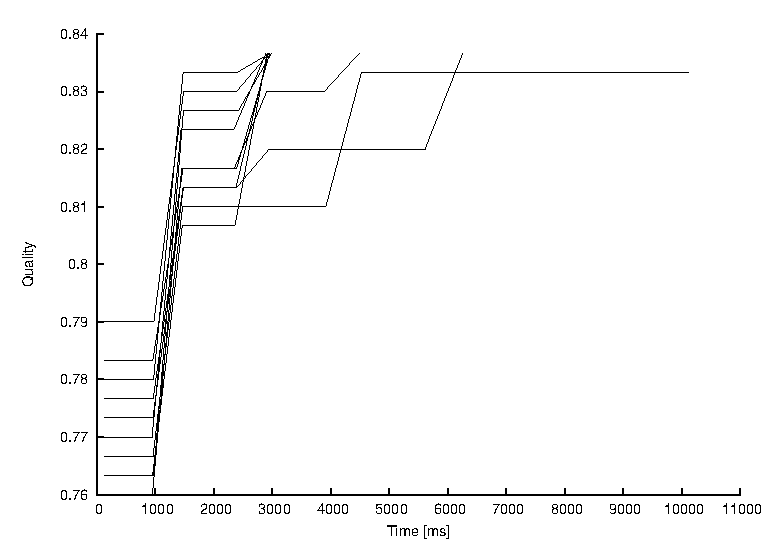
\includegraphics[width=\textwidth]{images/experiments/chained-ihs-s2}
\end{figure}

\begin{figure}
  \caption{Chained IHs - \dataset{100-100} Results for Strategy 3}
  \label{image-experiment-chained-ihs-s3}
  \centering
    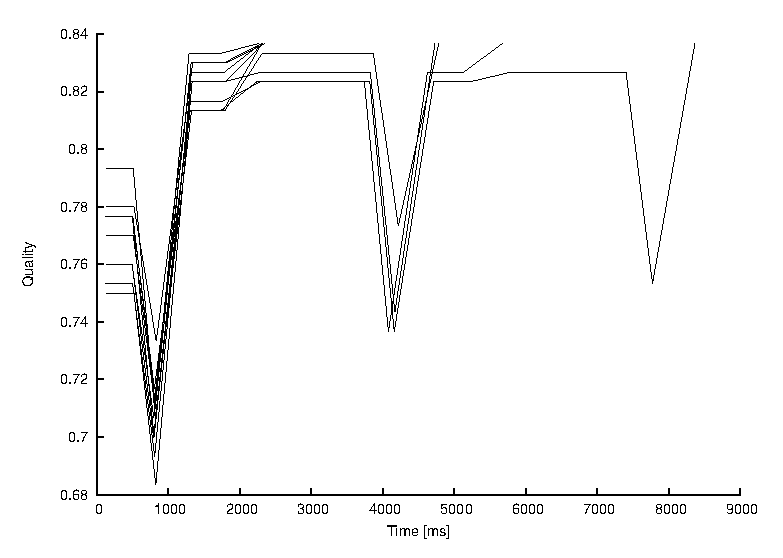
\includegraphics[width=\textwidth]{images/experiments/chained-ihs-s3}
\end{figure}

It is now necessary to assess which of the strategies perform the best. We shall take a look at the different data sets. Easily we can discard \dataset{MSH}, \dataset{NTH}, \dataset{XMA-c}, \dataset{XMA-p}, because the optimum is found in the very first step. Let us now introduce a metric for assessment of a strategy: namely, how many times of the 20 runs did it find the optimum. Results of this are summarized in Table \ref{table-experiments-chained-ihs-tweaking}.

\begin{table}
  \caption{Performance of Various IH Chains}
  \bigskip
  \label{table-experiments-chained-ihs-tweaking}
  \centering
  \begin{tabular}{l || c | c | c}
    Dataset & Strategy 1 & Strategy 2 & Strategy 3 \\
    \hline
    \dataset{100-100}  & \textbf{20} & 19 & \textbf{20} \\
    \dataset{100-200}  & \textbf{19} & 18 & 17 \\
    \dataset{100-1000} & 4  & 1  & \textbf{5}  \\
    \dataset{OVA1}     & \textbf{20} & \textbf{20} & \textbf{20} \\
    \dataset{OVA2}     & \textbf{19} & 13 & 18 \\
    \dataset{OVA3}     & 17 & 18 & \textbf{20} \\
    \end{tabular}
\end{table}

Each cell contains the number of times the strategy found optimum in the data set, out of 20 runs. Highlited are the strategies that performed best on that data set. We see that Strategy 1 and 3 are very similar in performance. We shall nonetheless choose Strategy \textbf{1} as the winner for its simplicity. Now we can tune its parameters.

\subsubsection{Improving Strategy 1}

%         NB class ChainedIHs1Tweak

A short reminder: Strategy 1 consists of \heu{Random} as the CH and the following IHs: \heu{RR} $\rightarrow$ \heu{MUT} $\rightarrow$ \heu{RR} $\rightarrow$ \heu{CX} $\rightarrow$ \heu{RW} $\rightarrow \ldots$

The parameters we can tune in this strategy are the ratios in \heu{RandomRemove} (possibly 2 of them, as there are 2 instances in use), \heu{Mutation} and \heu{Crossover}. We shall not tune the time limits in \heu{Mutation} and \heu{Crossover} and leave them set to 1 second. This presents us with a 3-dimensional space of parameters, where we want to find a combination best suited for our test data sets. We will sample this space by taking a total of 45 configurations of the aforementioned ratios.

\begin{center}
\bigskip
\begin{tabular}{| l | l |}
  \hline
  \hline
  Input data        & all sized test data sets \\
  Iterations        & 25 \\
  Pool size         & 10 \\
  $\alpha$, $\beta$ & $1$, $1$ \\
  CH                & \heu{Random} \\
  IHs               & \heu{RR} $\rightarrow$ \heu{MUT} $\rightarrow$ \heu{RR} $\rightarrow$ \heu{CX} $\rightarrow$ \heu{RW} $\rightarrow \ldots $ \\
  \hline
\end{tabular}
\bigskip
\end{center}

This experimental set will consist of 45 ratio combinations * 11 data sets * 25 iterations = 12375 experimental configurations. CH will be \heu{Random} with pool size of 10. IHs will be the ones from Strategy 1, with their ratios set to one of the 45 combinations produced in the following way.
\begin{itemize}
	\item \heu{RandomRemove} ratio will be from $\{0, 0.05, 0.1, 0.2, 0.5\}$
	\item \heu{Mutatio} ratio will be from $\{0.05, 0.1, 0.2\}$
	\item \heu{Crossover} ratio will be from $\{0.05, 0.1, 0.2\}$
\end{itemize}
The process of creating the configurations is captured in Listing \ref{listing-experiment-chained-ihs-tuning}. We will be gathering the following information for each run: what were the parameters, how long did the run take and whether it found optimum.\\

\begin{algorithm}
\caption{Chained IHs - Improving Strategy 1 Set Generation}
\label{listing-experiment-chained-ihs-tuning}
\begin{algorithmic}
\ENSURE experimental set $ES$
\STATE $ES \gets \emptyset$

\STATE $RW \gets \heu{RemoveWorst}$

\FOR{$rrRatio \in \{0, 0.05, 0.1, 0.2, 0.5\}$}
\FOR{$mutRatio \in \{0.05, 0.1, 0.2\}$}
\FOR{$cxRatio \in \{0.05, 0.1, 0.2\}$}
  \STATE $RR \gets \heu{RandomRemoval}(ratio = rrRatio)$
  \STATE $MUT \gets \heu{Mutation}(ratio = mutRatio, limit = 1)$
  \STATE $CX \gets \heu{Crossover}(ratio = cxRatio, limit = 1)$
  \FOR{$file \in $ sized test data}
    \FOR{$i = 1 \to 50$}
      \STATE $ES \gets ES \cup \{file, CH = \heu{Random}, IH = (\heu{RR}, \heu{MUT}, \heu{RR}, \heu{CX}, \heu{RW})\}$
    \ENDFOR
  \ENDFOR
\ENDFOR
\ENDFOR
\ENDFOR
\RETURN $ES$
\end{algorithmic}
\end{algorithm}

% TODO we ignore the time, instead we use the ratio of successful runs

After averaging the data we get a large result table, an excerpt from which is in Table \ref{table-experiments-chained-ihs-tweaking-s1}. In the left part are the ratio values, in the right part averaged running times for each data set. Highlited are the shortest times for each set. Only rows containing at least one such shortest time are presented.

% TODO replace this table

\begin{table}
  \caption{Performance of Strategy 1 Depending on Parameters - Excerpt}
  \bigskip
  \label{table-experiments-chained-ihs-tweaking-s1}
  \centering
  \begin{tabular}{c | c | c || c | c | c | c | c | c}
    \heu{RR} & \heu{MUT} & \heu{CX} & \dataset{100-100} & \dataset{100-1000} & \dataset{100-200} & \dataset{OVA1} & \dataset{OVA2} & \dataset{OVA3} \\
    \hline
    0.2	& 0.2	& 0.2	   & 2749.58	       & \textbf{8633.76} & 3029.82	         & 110.82	        & 98.68	         & 2413.86 \\
    0.5	& 0.05	& 0.05 & 1031.24	       & 10324.46	        & 1371.08	         & \textbf{71.88} & 63.86	         & 1282.94 \\
    0.5	& 0.05	& 0.2	 & \textbf{919.74} & 10978.58	        & 1322.02	         & 74.46	        & 62.42	         & \textbf{1217.00} \\
    0.5	& 0.1	& 0.2	   & 1002.20	       & 11030.64	        & \textbf{1288.06} & 85.22	        & 80.96	         & 1480.90 \\
    0.5	& 0.2	& 0.1	   & 1674.78	       & 9779.82	        & 2007.42	         & 108.14	        & \textbf{58.56} & 1827.46 \\
    \end{tabular}
\end{table}

% TODO the ratios actually are 0.5, 0.2 and 0.1, consistently across all all data sets

It is now necessary to pick one ratio combination as the best one. It is $(RR = 0.5, MUT = 0.05, CX = 0.2)$ for the following reason: it is the best one for sets \dataset{100-100} and \dataset{OVA3} and second best for \dataset{100-200}, \dataset{OVA1} and \dataset{OVA2}. Only the \dataset{100-1000} does not profit from these settings.

Now to interpret ratios in the best combination. \heu{RandomRemove} ratio of 0.5 means that a randomly chosen half of all AMs from every ID set in the pool will be discarded. This amounts to a very strong diversification tendency and keeps the strategy from stalling in local optima. \heu{Mutation} ratio of 0.05 means only around 5\% of AMs in the incumbent solution will be fixed for the next GLPK optimization. \heu{Crossover} ratio of 0.2 means that around 1/5\textsuperscript{th} of ID sets in the pool (randomly chosen) will be scanned for common AMs.

All of the ratios in the best combination are at one end of the range we chose from them. As a future work option it is possible to start moving these ratios even more in their preferred way, possibly removing \heu{Mutation} in the process.

TODO compare this to pure GLPK run - for example for \dataset{100-200}, we got from TODO seconds to on average TODO seconds (when the 10 second limit is lifted).

TODO this will need 2 boxplots again...

\begin{figure}
  \caption{Chained IHs - Pure \heu{Glpk} vs. Tuned Strategy 1}
  \label{image-experiment-chained-ihs-tuned}
  \centering
    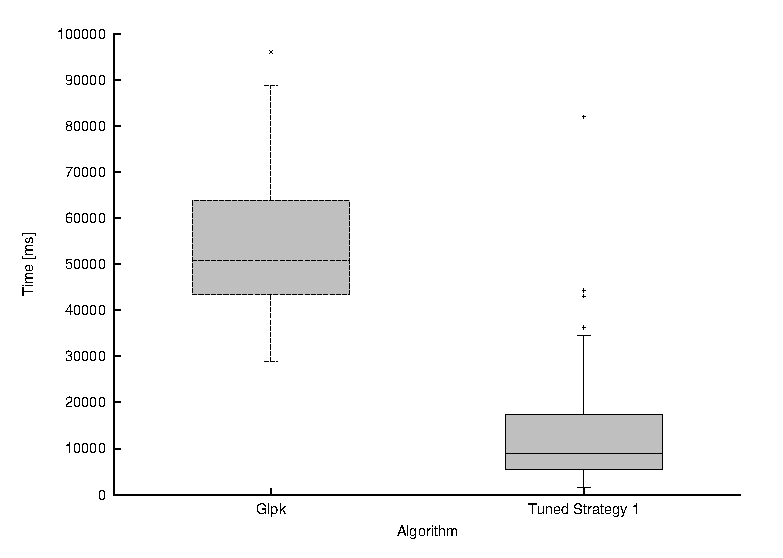
\includegraphics[width=\textwidth]{images/experiments/chained-ihs-tuned}
\end{figure}

\section{The "Best" Algorithm}

After asking and answering a lot of questions related to the overall system behavior, parameter effects and various heuristic combinations is now the time to summarize our results and draw conclusions.

The first fact is that if we have the time available, it is best to just let the GLPK run. It will find the optimum eventually, even though this might take minutes or hours to complete. For many purposes, this is just fine - we need to infer something about the schema, we do it only once, so it doesn't matter how long it takes.

Secondly, if we don't have enough time, or have to work in a dynamic environment, we should employ a metaheuristic with a series of improvement heuristics, more specifically Strategy 1. In under 10 seconds we will have very good results, often the optimum.

Overall, it is always good to ignore the simple text data nodes, as it will improve the total search time.

%\section{Lessons Learned}

%This short section will list a few lessons that were learned during the development of \jmodule{IDSetSearch} module for jInfer and experimenting with it.

%The first lesson is that when there is an experiment being run in a few nested loops (see any experiment set construction listing), one of which is \textit{iterations}, this one should be the outermost one. This is because if the experiment somehow fails, TODO

% - always allow for interruptions
% - when representing an object, don't be lazy and create a class for it (don't use pairs, lists with specific data at specific locations, etc)